\ifxHPTDC{
    \newcommand{\device}{}
    \newcommand{\deviceindex}{\cronvar{int}{index}}
    \newcommand{\deviceconfig}{}
    \newcommand{\initparameters}{xhptdc8\tu manager\tu init\tu parameters}
}{
    \newcommand{\device}{\cronvar{\prefix device}{*device}}
    \newcommand{\deviceindex}{\device}
    \newcommand{\deviceconfig}{\deviceindex, }
    \newcommand{\initparameters}{\prefix init\tu parameters}
}

The API is a DLL with C linkage.\par

The functions provided by the driver are declared in
\texttt{\txh{TimeTagger4}{xTDC4}{xHPTDC8}\tu interface.h} 
which must be included by your source code.
You must tell your compiler to link with the file
\ifxHPTDC{%
    \texttt{xhptdc8\tu driver.lib} or the corresponding 64 bit version
    \texttt{xhptdc8\tu driver\tu 64.lib}.
}{%
    \textsf{xTDC4\tu driver\tu 64.lib}.}
When running your program the dynamic link library containing the actual
driver code must reside in the same directory as your executable or be in a
directory included in the PATH variable. For Linux, it is provided only as a
static library \texttt{libxtdc4\tu driver.a} 
The file for the DLL is called \texttt{xTDC4\tu driver\tu 64.dll}.

All these files are provided with the driver installer that can be downloaded
from the product website \href{https://www.cronologic.de}{www.cronologic.de}. 
By default, the installer will place the files into the directory 
\texttt{C:\filesep Program Files\filesep cronologic\filesep \deviceName\filesep driver}.
A coding example can be found on\\
\href{https://github.com/cronologic-de/xtdc_babel/tree/main/timetagger4_user_guide_example}{github.com/cronologic-de/xtdc\_babel}.

\ifxHPTDC{
    There exist an open-source community project that intends to provide some
    convenient extensions to the driver, code examples, and wrappers to make
    the driver usable with various programming languages like Python and
    LabView. The project is hosted at
    \url{https://github.com/cronologic-de/xhptdc8_babel}.
}{}

 
\section{Constants}
\ifxHPTDC{
    \begin{description}[style=nextline]
        \item[\crondef{XHPTDC8\tu MANAGER\tu DEVICES\tu MAX 8}]
        The maximum number of boards supported by the device manager.

        \item[\ttdef{TDC\tu CHANNEL\tu COUNT 8}]
        The number of TDC input channels.

        \item[\ttdef{GATE\tu COUNT 8}]
        The number of gating blocks. One for each TDC input.

        \item[\ttdef{TIGER\tu COUNT 9}]
        The number of timing generators. One for each TDC input and one for the
        ADC trigger.

        \item[\ttdef{TRIGGER\tu COUNT 16}]
        The number of potential trigger sources for the timing generators. One
        for each TDC input \ifxHPTDC{}{, one for the Start input} plus some
        specials.  See Section~\ref{structtrigger} for details.
}{ 
    \begin{description}[style=nextline]
        \item[\ttdef{TDC\tu CHANNEL\tu COUNT 4}]
        The number of TDC input channels.

        \item[\ttdef{TIGER\tu COUNT 5}]
        The number of timing generators. One for each TDC input and one for the
        start input.

        \item[\ttdef{TRIGGER\tu COUNT 16}]
        The number of potential trigger sources for the timing generators. One
        for each TDC input, one for the Start input plus some specials. See
        Section~\ref{cp:tigerblock} for details. 
}
    \item[\ttdef{OK 0}]
    Error codes are set by the API functions to this value if there has
    been no error. Other error codes can be found in
    \texttt{\txh{TimeTagger4}{xTDC4}{xHPTDC8}\tu interface.h}
\end{description}





\section{Driver Information}
Even if there is no board present the driver revision can be queried using
these functions.

\begin{description}[style=nextline]
    \item[\ttvar{int}{get\tu driver\tu revision()}]
    Returns the driver version, same format as \texttt{\prefix static\tu
    info.driver\tu revision}.  This function does not require \adeviceName\
    board to be present.

    \item[\ttvar{const char*}{get\tu driver\tu revision\tu str()}]
    Returns the driver version including SVN build revision as a string. 

    \item[\ttvar{int}{count\tu devices(}\cronvar{int}{*error\tu code},
    \cronvar{char}{**error\tu message)}\label{countdevices}]
    Returns the number of boards present in the system that are supported by
    this driver.  Pointers to an error code and message variable have to be
    provided. If {\ttfamily error\_code} does not equal
    {\ttfamily\ttdef{OK} = 0}, the error message will contain what went wrong.
    E.g., crono kernel was not properly installed. \par
\end{description}




\section{Initialization}
The card must be initialized first before reading data. Normally the process is
to get the default init parameters and change some values. E.g., choose one of
multiple cards by the index or use a larger buffer.
    

\begin{description}[style=nextline]
    \item[\ttvar{int}{get\tu default\tu init\tu
        parameters(}\cronvar{\initparameters}{*init)}]
    Sets up the standard parameters. Gets a set of default parameters for
    \texttt{\prefix init()}.  This must always be used to initialize the
    \texttt{\initparameters} structure before modifying it and passing it to
    \texttt{\prefix init}.

    \ifxHPTDC{
        \item[\ttvar{int}{init(}\cronvar{\initparameters}{*params})]
    }{
        \item[\cronvar{\prefix device}{\prefix
            init(}\cronvar{\initparameters}{*params}, \cronvar{int}{*error\tu
            code}, \cronvar{char}{**error\tu message)}]
    }
    Opens and initializes the \deviceName\ 
    \ifxHPTDC{boards in the system}{board with the given index}. \par
    \ifxHPTDC{
        If the return value does not equal {\ttfamily\ttdef{OK} = 0}
        the device initialization failed.
    }{
        \texttt{error\tu code} must point to an integer where the driver can 
        write the error code.\par
        \texttt{error\tu message} must point to a pointer to char.  The driver
        will allocate a buffer for zero-ter\-mi\-na\-ted error message and 
        store the address of the buffer in the location provided by the
        user.\par
    }
    The parameter \texttt{params} is a pointer to a structure of
    type \texttt{\initparameters} that must be completely initialized by
    \texttt{get\tu default\tu init\tu parameters()}.

    \item[\ttvar{int}{close(}\device )]
    Closes the devices, releasing all resources. 
\end{description}

%%%%%%%%%%%%%%%%% struct init_parameters

\subsection{Structure \initparameters}
\begin{description}[style=nextline]
    \item[\cronvar{int}{version}\txhinits{}{}{\PREFIX API\tu VERSION}]
    The version number. Must be set to \texttt{\PREFIX API\tu VERSION}.\par

    \ifxHPTDC{}{
        \item[\cronvar{int}{card\tu index}]
        The index in the list of \deviceName\ boards that should be
        initialized.\par
        There might be multiple boards in the system that are handled by this
        driver as reported by \texttt{\prefix count\tu devices}. This index
        selects one of them. Boards are enumerated depending on the PCIe slot.
        The lower the bus number and the lower the slot number the lower the
        card index.

        \item[\cronvar{int}{board\tu id}]
        The global index in all cronologic devices.\par
        This 8-bit number is filled into each packet created by the board and
        is useful if data streams of multiple boards will be merged. If only
        \deviceName\ cards are used this number can be set to the
        \texttt{card\tu index}.  If boards of different types that use a
        compatible data format are used in a system each board should get a
        unique id.  Can be changed with \texttt{int \prefix set\tu board\tu
        id\allowbreak(\prefix device *device, int board\tu id)}.}


    \item[\cronvar{uint64\tu t}{buffer\tu size\ifxHPTDC{}{[8]}}%
        \txhinits{}{}{XHPTDC\_DEFAULT\_BUFFER\_SIZE}%
        \txh{}{}{\normalfont\ttfamily\ // 0x1000000 (16 MB)}]
    The minimum size of the DMA buffer.\\
    If set to \texttt{0} the default size of 16\,MByte is used. 
    \ifxHPTDC{}{For the \deviceName\ only the first entry is used.}\par

    \ifxHPTDC{}{
        \item[\cronvar{int}{buffer\tu type}]
        The type of buffer. Must be set to \texttt{0}.
        \begin{description}
            \item[]  \ttdef{BUFFER\tu ALLOCATE   0}
            \item[]  \ttdef{BUFFER\tu USE\tu PHYSICAL   1}  // unsupported
        \end{description}

        \item[\cronvar{uint64\tu t}{buffer\tu address}]
        This is set by \texttt{\prefix init()} to the start address of the
        reserved memory.\par
        The buffers will be allocated with the sizes given above. Make sure
        that the memory is large enough.
    }

    \item[\cronvar{int}{variant}\txhinits{0}{0}{0}]
    Set to \texttt{0}. Can be used to activate future device variants such as
    different base frequencies.\par

    \item[\cronvar{int}{device\tu type}\txhinits{}{}{CRONO\_DEVICE\_XHPTDC8}]
    A constant for the different devices of cronologic
    \texttt{CRONO\tu DEVICE\tu *}.\par
    Initialized by \texttt{\prefix get\tu default\tu init\tu parameters()}.
    This value is identical to the PCI Device ID. Must be left unchanged.

    \begin{tabular}{ll}
        \crondef{CRONO\tu DEVICE\tu HPTDC}       & \ttfamily 0x1 \\
        \crondef{CRONO\tu DEVICE\tu NDIGO5G}     & \ttfamily 0x2 \\
        \crondef{CRONO\tu DEVICE\tu NDIGO250M}   & \ttfamily 0x4 \\
        \crondef{CRONO\tu DEVICE\tu xTDC4}       & \ttfamily 0x6 \\
        \crondef{CRONO\tu DEVICE\tu TIMETAGGER4} & \ttfamily 0x8 \\
        \crondef{CRONO\tu DEVICE\tu XHPTDC8}     & \ttfamily 0xC \\
        \crondef{CRONO\tu DEVICE\tu NDIGO6}      & \ttfamily 0xD \\
    \end{tabular}

    \item[\cronvar{int}{dma\tu read\tu delay}\txhinits{}{}{250}]
    The update delay of the write pointer after a packet has been sent over
    PCIe. Specified in multiples of \SI{16}{\nano\second}.  Should not be
    changed by the user.

    \ifxHPTDC{
        \item[\cronvar{crono\tu bool\tu t}{multiboard}\txhinits{}{}{false}]
        Set if multiple devices shall be synchronized. Also sets the clock
        source to external.

        \item[\cronvar{crono\tu bool\tu t}{use\tu ext\tu clock}%
            \txhinits{}{}{false}]
        If set use the external 10\,MHz reference on J2, otherwise the internal
        clock source is used.  When \texttt{multiboard} is set, this parameter
        is ignored and the external clock is used. 

        \item[\cronvar{crono\tu bool\tu t}{ignore\tu calibration}%
            \txhinits{}{}{false}]
        Leave at \texttt{false} to use device calibration data.

    }{
        \item[\cronvar{int}{use\tu ext\tu clock}]
        If set to \texttt{1}, use external 10\,MHz reference. If set to
        \texttt{0}, use internal reference.
    }
\end{description}

% info structures
\section{Status Information}
	

\subsection{Functions for Information Retrieval}
The driver provides functions to retrieve detailed information on the
board type, its configuration, settings, and state.  The information is
split according to its scope and the computational requirements to query
the information from the board.

\ifxHPTDC{
    The information is provided on a per board basis. The parameter
    \texttt{index} selects which board is queried.
}{}

\begin{description}[style=nextline]
    \item[\ttvar{int}{get\tu device\tu type}(\deviceindex)]
    Returns the type of the device as \texttt{CRONO\tu DEVICE\tu
    \txh{TIMETAGGER4}{XTDC4}{XHPTDC8}}.

    \item[\ttvar{const char*}{get\tu last\tu error\tu message(\deviceindex)}]
    Returns most recent error message.
    \ifxHPTDC{
        If index is negative the last error message from the \\
        \texttt{\prefix manager} is returned. Otherwise, the last error message
        of the selected board is returned.
    }{}

    \item[\ttvar{int}{get\tu fast\tu info(}\deviceindex, \cronvar{\prefix fast\tu info}{*info)}]
    Returns fast dynamic information.\par
    This call gets a structure that contains dynamic information that can be
    obtained within a few microseconds.

    \item[\ttvar{int}{get\tu param\tu info(}\deviceindex, \cronvar{\prefix param\tu info}{*info)}]
    Returns configuration changes.\par
    Gets a structure that contains information that changes indirectly due to
    configuration changes.


    \item[\ttvar{int}{get\tu static\tu info(}\deviceindex, \cronvar{\prefix static\tu info}{*info)}]
    Contains static information.\par
    Gets a structure that contains information about the board that does not
    change during run time.

    \ifxHPTDC{
        \item[\ttvar{int}{get\tu temperature\tu info(}\deviceindex, \cronvar{\prefix temperature\tu info}{*info)}]
        Get temperature measurements from multiple sources on the board.

        \item[\ttvar{int}{get\tu clock\tu info(}\deviceindex, \cronvar{\prefix
            clock\tu info}{*info)}]
        Get information on clocking configuration and status.

        \item[\ttvar{const char*}{device\tu state\tu to \tu str(}\cronvar{int}{state)}]
        Convert the state value from \texttt{\prefix fast\tu info.state} into
        a human-readable string. 
    }{} 
\end{description}

%%%%%%%%%%%%%%%%% static info

\subsection{Structure \prefix static\tu info}

This structure contains information about the board that does not change during
run time. It is provided by the function
\texttt{\prefix get\tu static\tu info()}.

\begin{description}[style=nextline]
    \item[\cronvar{int}{size}]
    The number of bytes occupied by the structure.

    \item[\cronvar{int}{version}]
    A version number that is increased when the definition of the structure is
    changed. The increment can be larger than one to match driver version
    numbers or similar.

    \item[\cronvar{int}{board\tu id}]
    ID of the board.\par
    \ifxHPTDC{
        All \deviceName\ boards in the system are numbered in the order of
        their serial numbers starting at zero.  Channel A of a board has
        channel number $index \times 10$.
    }{}

    \item[\cronvar{int}{driver\tu revision}]
    Encoded version number for the driver.\par
    The lower three bytes contain a triple-level hierarchy of version numbers,
    e.g., \texttt{0x010103} encodes version 1.1.3.\par
    The version adheres to the Semantic Versioning scheme as defined at
    \href{https://semver.org}{https://semver.org}. A change in the first digit
    generally requires a recompilation of user applications.  Changes in the
    second digit denote significant improvements or changes that don't break
    compatibility and the third digit increments with minor bug fixes and
    similar updates that do not affect the API.

    \item[\cronvar{int}{driver\tu build\tu revision}]
    Build number of the driver according to cronologic's internal versioning
    system.

    \item[\cronvar{int}{firmware\tu revision}]
    Revision number of the FPGA configuration.

    \item[\cronvar{int}{board\tu revision}]
    Board revision number.\par
    The board revision number can be read from a register. It is a four-bit
    number that changes when the schematic of the board is changed. This should
    match the revision number printed on the board.

    \item[\cronvar{int}{board\tu configuration}]
    Describes the schematic configuration of the board.\par
    The same board schematic can be populated in multiple variants. This is an
    8-bit code that can be read from a register.

    \item[\cronvar{int}{subversion\tu revision}]
    Subversion revision id of the FPGA configuration source code.

    \txh{
        \item[\cronvar{int}{chip\tu id}]
        Reserved.
    }{
        \item[\cronvar{int}{chip\tu id}]
        16 bit factory ID of the TDC chip.
    }{
        \item[\cronvar{int}{chip\tu id[2]}]
        16 bit factory ID for each of the TDC chips.
    }

    \item[\cronvar{int}{board\tu serial}]
    Serial number.\par
    Year and running number are concatenated in 8.24 format. The number is
    identical to the one printed on the silvery sticker on the board.

    \item[\protect{\parbox[b]{0.8\linewidth}{
        \cronvar{\uint}{flash\tu serial\tu high}\\
        \cronvar{\uint}{flash\tu serial\tu low}}}]
    64-bit manufacturer serial number of the flash chip

    \item[\cronvar{crono\tu bool\tu t}{flash\tu valid}]
    If not \texttt{0}, the driver found valid calibration data in the flash on
    the board and is using it. This value is not applicable for the
    \deviceName.

    \item[\cronvar{char}{calibration\tu date[20]}]
    DIN EN ISO 8601 string YYYY-MM-DD HH:MM of the time when the card
    was calibrated.

    \item[\cronvar{char}{bitstream\tu date[20]}]
    DIN EN ISO 8601 string YYYY-MM-DD HH:MM of the time when the bitstream on
    the card was created.

    \txh{
        \item[\cronvar{double}{delay\tu bin\tu size}]
        Bin size of delay in picoseconds. The increment of the
        \texttt{delay\tu config.delay} field for the \deviceName.

        \item[\cronvar{double}{auto\tu trigger\tu ref\tu clock}]
        Auto trigger clock frequency. The clock frequency of the auto trigger
        in Hertz used for calculating the \texttt{auto\tu trigger\tu period}.

        \item[\cronvar{uint32\tu t}{rollover\tu period}]
        The number of bins in a rollover period. This is a power of 2 (the
        maximum value of a hit timestamp is this value minus 1)
    }{}{}
\end{description}

%%%%%%%%%%%%%%%%%%%%%%%% param info
\subsection{Structure \prefix param\tu info}
This structure contains configuration changes provided by \texttt{\prefix
get\tu param\tu info()}.

\begin{description}[style=nextline]
    \item[\cronvar{int}{size}]
    The number of bytes occupied by the structure.

    \item[\cronvar{int}{version}]
    A version number that is increased when the definition of the structure is
    changed. The increment can be larger than one to match driver version
    numbers or similar.

    \item[\cronvar{double}{binsize}]
    Bin size (in \si{\pico\second}) of the measured TDC data.

    \ifxHPTDC{}{ %board ID is found in the static_info structure for .
        \item[\cronvar{int}{board\tu id}]
        Board ID.\par
        The board uses this ID to identify itself in the output data stream.
        The ID takes values between \texttt{0} and \texttt{255}.
    }

    \item[\cronvar{int}{channels}]
    Number of TDC channels of the board.\par
    Fixed at \texttt{\ifxHPTDC{8}{4}}.

    \item[\cronvar{int}{channel\tu mask}]
    Bit assignment of each enabled input channel.\par
    Bit $\texttt{0} \leq n < \texttt{\ifxHPTDC{8}{4}}$ is set if channel $n$ is
    enabled.

    \item[\cronvar{int64\tu t}{total\tu buffer}]
    The total amount of DMA buffer in bytes.

    \ifxHPTDC{}{
        \item[\cronvar{double}{packet\tu binsize}]
        \itett{ %tt4
            For the \deviceName\, the packet binsize is equal to the binsize
            and depends on the generation of the card. Gen\,1 boards have a
            packet binsize of \SI{500}{\pico\second}, while Gen\,2 boards have
            \SI{100}{\pico\second}.
        }{ %xtdc4
            For \deviceName\, this is \SI{1666.6}{\pico\second}
        }
    }

    \ifxHPTDC{}{
        \item[\cronvar{double}{quantisation}]
        \itett{ %tt4
            Quantisation or measurement resolution. Depending on the board
            variant this ranges from \SIrange{100}{1000}{\pico\second}.\par
            \begin{tabular} {|l|l|l|l|l|l|l}
            \hline
            --1G & --2G & --1.25G & --2.5G & --5G & --10G \\
            \hline
            1000 ps & 500 ps & 800 ps & 400 ps & 200 ps & 100 ps\\
            \hline
            \end{tabular}

            This means, that for --1.25G the lower 3 bits in the timestamps are
            zero.
        }{ %xtdc4
            Quantisation or measurement resolution. For the \deviceName\, this
            is \SI{13.0208}{\pico\second}
        }
    }
\end{description}

%%%%%%%%%%%%%%%%%%%%%%%%%% fast info

\subsection{Structure \prefix fast\tu info} \label{structfastinfo}
\begin{description}[style=nextline]
    \item[\cronvar{int}{size}]
    The number of bytes occupied by the structure. 

    \item[\cronvar{int}{version}]
    A version number that is increased when the definition of the structure is
    changed.  The increment can be larger than one to match driver version
    numbers or similar.

    \ifxHPTDC{} {
        \item[\cronvar{int}{tdc\tu rpm}]
        Speed of the TDC fan in rounds per minute. Reports \texttt{0} if no fan
        is present.
    }

    \item[\cronvar{int}{fpga\tu rpm}]
    Speed of the FPGA fan in rounds per minute. Reports \texttt{0} if no fan is
    present.

    \item[\cronvar{int}{alerts}]
    Alert bits from the temperature sensor and the system monitor.
    \itett{
        The TimeTagger4 does not implement any temperature alerts.
    }{
        Bit 0 is set if the TDC temperature exceeds \SI{140}{\degreeCelsius}. 
        In this case the TDC did shut down and the device needs to be
        reinitialized. 
    }

    \item[\cronvar{int}{pcie\tu pwr\tu mgmt}]
    Always \texttt{0}.

    \item[\cronvar{int}{pcie\tu link\tu width}]
    Number of PCIe lanes the card uses. Should always be \texttt{10} for the
    \deviceName.

    \item[\cronvar{int}{pcie\tu max\tu payload}]
    Maximum size in bytes for one PCIe transaction. Depends on system
    configuration.

    \ifxHPTDC{
    \item[\cronvar{int}{state}]
    Current state of the \deviceName. 

    \begin{tabular}{lc}
        \cronvar{const static int}{\PREFIX DEVICE\tu STATE\tu CREATED} & \texttt{0}  \\*
        \cronvar{const static int}{\PREFIX DEVICE\tu STATE\tu INITIALIZED} & \texttt{1}  \\*
        \cronvar{const static int}{\PREFIX DEVICE\tu STATE\tu CONFIGURED} & \texttt{2}  \\*
        \cronvar{const static int}{\PREFIX DEVICE\tu STATE\tu CAPTURING} & \texttt{3}  \\*
        \cronvar{const static int}{\PREFIX DEVICE\tu STATE\tu PAUSED} & \texttt{4}  \\*
        \cronvar{const static int}{\PREFIX DEVICE\tu STATE\tu CLOSED} & \texttt{5}  \\*
    \end{tabular}
    }{}
\end{description}
%%%%%%%%%%%%%%%%%%%%%%% temperature info

\ifxHPTDC{
    \subsection{Structure \prefix temperature\tu info}
    This structure provide the values of temperature measurements of
    various chips on the board.

    \begin{description}[style=nextline]
        \item[\cronvar{int}{size}]
        The number of bytes occupied by the structure.

        \item[\cronvar{int}{version}]
        A version number that is increased when the definition of the
        structure is changed. The increment can be larger than one to match
        driver version numbers or similar.

        \item[\cronvar{float}{tdc[2]}]
        Temperature for each of the TDC chips in \si{\degreeCelsius}.
    \end{description}

    %%%%%%%%%%%%%%%%%%%%% clock info

    \subsection{Structure \prefix clock\tu info}
    This structure provides information about the clock network of the
    device. 

    \begin{description}[style=nextline]
        \item[\cronvar{int}{size}]
        The number of bytes occupied by the structure.

        \item[\cronvar{int}{version}]
        A version number that is increased when the definition of the structure
        is changed. The increment can be larger than one to match driver
        version numbers or similar.\par

        \item[\cronvar{crono\tu bool\tu t}{cdce\tu locked}]
        Set if the jitter cleaning PLL clock synthesizer achieved lock.

        \item[\cronvar{int}{cdce\tu version}]
        Version information from the CDCE62005 clock synthesizer.
        
        \item[\cronvar{crono\tu bool\tu t}{use\tu ext\tu clock}]
        Source for the clock synthesizer is usually the 10~MHz onboard
        oscillator. During initialization, alternatively an external clock
        on J2 can be selected.  When multiple boards are synchronized all board
        use a common external clock. See section \ref{multiboard} for details.
    
        \item[\cronvar{crono\tu bool\tu t}{fpga\tu locked}]
        Set if the FPGA datapath PLL achieved lock.
    \end{description}
}{}



\section{Configuration}
\ifxHPTDC{
    All \deviceName\ boards in the system are configured by a single
    configuration structure which in turn contains sub structures that
    configure the individual boards.
}{
    The device is configured with a configuration structure.
}
The user should first obtain a structure that contains the default settings of
the device read from an on-board ROM, then modify the structure as needed for
the user application and use the result to configure the device.\par

\begin{description}[style=nextline]
    \item[\ttvar{int}{configure(}\deviceconfig\cronvar{\prefix\ifxHPTDC{manager\tu }{}configuration}{*config)}]
    Configures the \texttt{\prefix manager}.

    \item[\protect{\parbox[b]{1.0\linewidth}{
        \ttvar{int}{get\tu current\tu configuration(}\deviceconfig
        \ifxHPTDC{}{\hspace*{\labelwidth+\itemsep}}\cronvar{
            \prefix\ifxHPTDC{manager\tu }{}configuration}{\textbf{*config})}}}]
    Gets current configuration. Copies the current configuration to the
    specified config pointer.

    \item[\protect{\parbox[b]{1.0\linewidth}{
        \ttvar{int}{get\tu default\tu configuration(}\deviceconfig
        \ifxHPTDC{}{\hspace*{\labelwidth+\itemsep}}\cronvar{
            \prefix \ifxHPTDC{manager\tu}{}configuration}{\textbf{*config})}}}]
    Gets default configuration. Copies the default configuration to the
    specified config pointer.
\end{description}

\ifxHPTDC{
    \subsection{YAML config files}
    \label{yaml}
    There exist a community maintained utility library for the \deviceName\
    that contains a convenience function that can modify configuration
    structures from a YAML config string. This can significantly shorten code
    required to setup the TDC. \par
    See \href{https://github.com/cronologic-de/xhptdc8_babel/tree/main/util}{
        github.com/cronologic-de/xhptdc8\tu babel/tree/main/util} for details.  
}{} 

%%%%%%%%%%%%%%%%% configuration structure mostly shared between devices
%%%%%%%%%%%% struct manager configuration
\ifxHPTDC{
    \subsection{Structure \prefix manager\tu configuration}
    \begin{description}[style=nextline]
    \item[\cronvar{int}{size}]
    The number of bytes occupied by the structure.\par

    \item[\cronvar{int}{version}]
    A version number that is increased when the definition of the structure is
    changed. The increment can be larger than one to match driver version
    numbers or similar.\par

    \item[\cronvar{\prefix device\tu configuration}{device\tu
        configs[\PREFIX DEVICES\tu MAX]}]
    A structure with the configuration for an individual \deviceName\ board as
    defined in section \ref{structconfig}.  Use the function \texttt{\prefix
    count\tu devices()} to query how many entries contain valid information.
    See Section~\ref{countdevices} for details on the function.

    \item[\cronvar{\prefix grouping\tu configuration}{grouping}]
    Structure with the parameters for grouping. \par
    See Section~\ref{structgrouping} for the definition of the structure and
    Section~\ref{sec:grouping} for more information on grouping.

    \item[\cronvar{\longlong}{*bin\tu to\tu ps(\longlong)}]
    Reserved for future use.
    \end{description}
}{}
%%%%%%%%%%%%%% struct device_configuration
\subsection{Structure \prefix \ifxHPTDC{device\tu}{}configuration}
\label{structconfig}
This is the structure containing the configuration information.
\ifxHPTDC{}{ % xHPTDC8 uses TDC manager instead
    It is used in conjunction with \texttt{\prefix get\tu default\tu
    configuration()}, \texttt{\prefix get\tu current\tu configuration()} and
    \texttt{\prefix configure()}.\par
}
It uses multiple substructures to configure various aspects of the board.

\begin{description}[style=nextline]
    \item[\cronvar{int}{size}]
    The number of bytes occupied by the structure.\par

    \item[\cronvar{int}{version}]
    A version number that is increased when the definition of the structure is
    changed. The increment can be larger than one to match driver version
    numbers or similar.\par

    \ifxHPTDC{
        \item[\protect{\parbox[b]{\linewidth}{
            \cronvar{int}{auto\tu trigger\tu period}\txhinits{}{}{300000000}\\
            \cronvar{int}{auto\tu trigger\tu random\tu exponent}%
                \txhinits{}{}{0}}}]
        Create a trigger either periodically or randomly. There are two
        parameters
        \begin{align*}
        M &= \texttt{auto\tu trigger\tu period} \\
        N &= \texttt{random\tu exponent}
        \end{align*}
        that result in a distance between triggers of $T$ clock cycles.

        \begin{align*}
            T &= 1 + M + [1...2^N]\\
            0 &\leq M < 2^{32}\\
            0 &\leq N < 32
        \end{align*}

        \noindent There is no enable or reset. The auto-trigger is running
        continuously. The usage of this trigger can be configured in the
        TiGer block source field.\par
    }{}

    \ifxHPTDC{} %see xhptdc8_grouping_configuration.enable
    {
        \item[\cronvar{int}{tdc\tu mode}]
        TDC mode. Can be grouped or continuous defined as follows:\par
        \begin{tabular}{ll}
            \ttdef{TDC\tu MODE\tu GROUPED} & \texttt{0}\\
            \ttdef{TDC\tu MODE\tu CONTINUOUS} & \texttt{1}\\
        \end{tabular}\par
        \itett{
            \begin{itemize}
                \item Grouped functionality is explained in
                    Section~\ref{sec:grouping}.  
                \item Continuous mode is explained in
                    Section~\ref{cp:continousmode}. The
                    \texttt{auto\tu trigger\tu period} needs to be set
                    appropriately and \texttt{channel[i].stop} must be larger
                    than \texttt{auto\tu trigger\tu period} (respecting
                    the different periods or can be set to maximum of
                    \texttt{0xFFFFFFFF}), if all events need to be captured.
                \end{itemize}
        }{
            \begin{itemize}
                \item Grouped functionality is explained in
                    Section~\ref{sec:grouping}.  
                \item Not applicable for the \deviceName.              
            \end{itemize}
        }
    }

    \ifxHPTDC{} % does not exist for xHPTDC8
    {
        \item[\cronvar{crono\tu bool\tu t}{start\tu rising}]
        \itett{
            Not applicable for the \deviceName. Rising and/or falling edge
            are configured using the \texttt{\prefix trigger} structure
            (see Section~\ref{structtrigger}).
        }{
            Selects whether the rising or falling edge of the start signal
            is used to start a group.
        }
    }

    \label{apidcoffset}
    \ifxHPTDC{
        \item[\cronvar{double}{trigger\_threshold[\PREFIX TDC\tu CHANNEL\tu COUNT]}%
            \txhinits{}{}{-0.35}]
        Set the threshold voltage for the input channels
        \ifxHPTDC{A \ldots H}{S, A \ldots D} (see Figure~\ref{fig:dcoffset1}).
    }{
        \item[\cronvar{double}{dc\tu offset[\PREFIX TDC\tu
            CHANNEL\tu COUNT + 1]}]
        Set the threshold voltage for the input channels
        \ifxHPTDC{A \ldots H}{S, A \ldots D} (see Figure~\ref{fig:dcoffset1}).
        \begin{itemize}
            \item dc\tu offset[0] : threshold for channel Start
            \item dc\tu offset[1 - 4] : threshold for channels A \ldots D
        \end{itemize}
    }

    The supported range is \dcmin{} to \dcmax{}\,V. This should be close to 50\% of the height of the input pulse. Examples for various signaling standards are defined as follows:\par

    \ifxHPTDC{}{
        \textbf{Important Note:} The supported range changed for \hyperref[sec:rev_driver_applications]{driver release} 1.10.7. That means, if you use a value for \texttt{dc\_offset} outside the new supported range in your source code, the device configuration will report an error. Adjust your \texttt{dc\_offset} accordingly, preferably using the defines provided below.
    }

\ifxHPTDC{
    \newcommand{\DCOFFSET}{THRESHOLD\tu}
}{
    \newcommand{\DCOFFSET}{DC\tu OFFSET\tu}
}
    \begin{xltabular}{\textwidth}{ll}
        \ttdef{\DCOFFSET P\tu NIM} & \texttt{+0.35}\\
        \ttdef{\DCOFFSET P\tu CMOS} & \texttt{+\dcmax}\\
        \ttdef{\DCOFFSET P\tu LVCMOS\tu 33} & \texttt{+\dcmax}\\
        \ttdef{\DCOFFSET P\tu LVCMOS\tu 25} & \texttt{+\dcmax}\\
        \ttdef{\DCOFFSET P\tu LVCMOS\tu 18} & \texttt{+0.90}\\
        \ttdef{\DCOFFSET P\tu TTL} & \texttt{+\dcmax}\\
        \ttdef{\DCOFFSET P\tu LVTTL\tu 33} & \texttt{+\dcmax}\\
        \ttdef{\DCOFFSET P\tu LVTTL\tu 25} & \texttt{+\dcmax}\\
        \ttdef{\DCOFFSET P\tu SSTL\tu 3} & \texttt{+\dcmax}\\
        \ttdef{\DCOFFSET P\tu SSTL\tu 2} & \texttt{+\dcmax}\\
        \ttdef{\DCOFFSET N\tu NIM} & \texttt{-0.35}\\
        \ttdef{\DCOFFSET N\tu CMOS} & \texttt{-\dcminabs}\\
        \ttdef{\DCOFFSET N\tu LVCMOS\tu 33} & \texttt{-\dcminabs}\\
        \ttdef{\DCOFFSET N\tu LVCMOS\tu 25} & \texttt{-1.25}\\
        \ttdef{\DCOFFSET N\tu LVCMOS\tu 18} & \texttt{-0.90}\\
        \ttdef{\DCOFFSET N\tu TTL} & \texttt{-\dcminabs}\\
        \ttdef{\DCOFFSET N\tu LVTTL\tu 33} & \texttt{-\dcminabs}\\
        \ttdef{\DCOFFSET N\tu LVTTL\tu 25} & \texttt{-1.25}\\
        \ttdef{\DCOFFSET N\tu SSTL\tu 3} & \texttt{-\dcminabs}\\
        \ttdef{\DCOFFSET N\tu SSTL\tu 2} & \texttt{-1.25}\\
    \end{xltabular}\par
    \noindent The inputs are AC coupled. Thus, the absolute voltage is not
    important for pulse inputs.  It is the relative pulse amplitude that
    causes the input circuits to switch.  The parameter must be set to the
    relative switching voltage for the input standard in use.  If the pulses
    are negative, a negative switching threshold must be set and vice versa. 
    \begin{figure}
        \centering
        \ifxHPTDC{
            \includegraphics[width=0.3\textwidth]{
                xhptdc/figures/InputCircuit.pdf}
        }{
            \includegraphics[width=0.3\textwidth]{
                figures/InputCircuit.pdf}
        }
        \caption{Input circuit for each of the input channels.
            \label{fig:dcoffset1}}
    \end{figure}

	\txh{}{\clearpage}{\newpage} % pagebreak just for xTDC4 and HPTDC
    \item[\cronvar{\prefix trigger}{trigger[\PREFIX TRIGGER\tu COUNT]}]
    Configuration of the polarity of the external trigger sources (see
    Section~\ref{structtrigger}). These are used as inputs for the TiGer blocks
    and as inputs to the time measurement unit.

    \item[\cronvar{\prefix tiger\tu block}{
        tiger\tu block[\PREFIX TIGER\tu COUNT]}]
    Configuration of the timing generators (TiGer, see
    Section~\ref{cp:tigerblock}).
    \ifxHPTDC{
        \par Indices 0 through 7 refer to channels A through H; index 8
        to channel TRG.
    }{
        \par Index 0 refers to the Start channel; indices 1 through 4 to the
        Stop channels A through D.
    }

    \ifxHPTDC{ % only for xHPTDC8
        \label{member:gating_block}
        \item[\cronvar{\prefix tiger\tu block}{
            gating\tu block[\PREFIX GATE\tu COUNT]}]
        Configuration of the gating blocks.
    }{}

    \item[\cronvar{\prefix channel}{channel[\PREFIX TDC\tu CHANNEL\tu COUNT]}]
        Configuration of the TDC channels.

    \ifxHPTDC{
        \item[\cronvar{\prefix adc\_channel}{adc\tu channel}]
        Configuration of the ADC channel.

        \item[\cronvar{crono\tu bool\tu t}{skip\tu alignment}%
            \txhinits{}{}{false}]
        If set, the phase of the two TDC chips is not realigned when capturing
        is restarted.

        \item[\cronvar{int}{alignment\tu source}%
            \txhinits{}{}{1}]
        Define a signal source that is used for phase alignment. Should
        usually be left unchanged.\par
        \begin{tabular}{ll}
            \ttdef{ALIGN\tu TIGER}    & \texttt{0}\\
            \ttdef{ALIGN\tu PIN}      & \texttt{1}\\
            \ttdef{ALIGN\tu RESERVED} & \texttt{2}\\
        \end{tabular}\par

        \item[\cronvar{int}{alignment\_off\_state}\txhinits{}{}{0}]
        Select TDC alignment pin state when not in use.\par
        \begin{tabular}{ll}
            \texttt{0} & GND\\
            \texttt{1} & VCCIO\\
            \texttt{2} & high-Z\\
        \end{tabular}
    }{
        \item[\protect{\parbox[b]{\linewidth}{
            \ttvar{\prefix lowres\tu channel\\\hspace*{\labelwidth+\itemsep}}{%
            lowres\tu channel[\PREFIX LOWRES\tu CHANNEL\tu COUNT]}}}]
        \itett{
            Not applicable for the \deviceName.
        }{
            Only applicable to the xTDC4-S. Configures the additional
            digital low-res inputs.
        }
        \item[\protect{\parbox[b]{\linewidth}{
            \cronvar{uint32\tu t}{auto\tu trigger\tu period}\\
            \cronvar{uint32\tu t}{auto\tu trigger\tu random\tu exponent}}}]
        Create a trigger either periodically or randomly. There are two
        parameters
        \begin{align*}
            M &= \texttt{auto\tu trigger\tu period} \\
            N &= \texttt{random\tu exponent}
        \end{align*}
        that result in a distance between
        triggers of $T$ clock cycles.

        \itett{ %TT4
            If the autotrigger is used for the continuous mode the following
            boundaries apply. 
            \begin{align*}
                T &= M + [1...2^N] - 1\\
                31 &\leq M < 78\,125\,000\\
                0 &\leq N < 32
            \end{align*}

            Otherwise, the parameters can be used with the following boundaries.
            \begin{align*}
                T &= M + [1...2^N] - 1\\
                M_{\mathrm{min}} &\leq M < 2^{32}\\
                0 &\leq N < 32
            \end{align*}
            where $M_{\mathrm{min}}$ is 6 for Gen\,1 and 8 for Gen\,2.
       }{%xTDC4        
            \begin{align*}
                T &= M + [1...2^N] - 1\\
                6 &\leq M < 2^{32}\\
                0 &\leq N < 32
            \end{align*} 
        }
        \noindent There is no enable or reset. The auto-trigger is running
        continuously.  The usage of this trigger can be configured in the
        TiGer block source field.
    }
    \ifxHPTDC{}{
        \itett{
            \item[\protect{\parbox[b]{\linewidth}{
            \ttvar{\prefix delay\tu config\\\hspace*{\labelwidth+\itemsep}}{%
                delay\tu config[\PREFIX TDC\tu CHANNEL\tu COUNT+1]}}}]
            Configuration of the channel delay values

            \item[\cronvar{uint32\_t}{ignore\_empty\_packets}]
            If enabled (any value but \texttt{0}), do not write empty packets
            to the output stream. Disabled by default.
        }{} %not applicable for xTDC4
    }
    \end{description}


%%%%%%%%% trigger
\subsection{Structure \prefix trigger}
\label{structtrigger}
For each input, this structure determines whether rising or falling edges on
the inputs create trigger events for the TiGer \ifxHPTDC{and gating }{}blocks.

\begin{description}[style=nextline]
    \item[\protect{\parbox[b]{0.8\linewidth}{
        \cronvar{crono\tu bool\tu t}{falling}\txhinits{}{}{true}\\
        \cronvar{crono\tu bool\tu t}{rising}\txhinits{}{}{false}}}]
    Select for which edges a trigger event is created inside the FPGA.
    \txh{ %TT4
        Set the corresponding flag for one of the edges or both edges when
        using the input with a TiGer.
    }{ %xTDC4
        The \deviceName can output measurements with a reduced bin size of
        $5/6$\,\si{\nano\second} = \SI{833.333}{\pico\second} for one or both
        edges of input signals.  See section \ref{difficulthits} for more
        information on hits with varying resolution.  Use \textsf{xTDC4\tu
        channel.rising} on page \pageref{structchannel} to select which edge
        is measured with full resolution.  The edge that is selected for full
        resolution measurement must also be enabled for low resolution
        measurement.
    }{ % HPTDC
        While the TDC can only measure either rising or falling edges, the
        gating blocks and the TiGer are more flexible.  Set the corresponding
        flag for one of the edges or both edges when using the input with a
        TiGer or gating block.
    }
\end{description}

%%%%% tiger_block
\subsection{Structure \prefix tiger\tu block}\label{cp:tigerblock}
See Section~\ref{cp:tiger} for additional information.

\begin{description}[style=nextline]
    \ifxHPTDC{
        \item[\cronvar{int}{mode}\txhinits{}{}{0}]
        Enables the desired mode of operation for the tiger.\par
        \begin{tabular}{lrl}
            \ttdef{TIGER \tu OFF}     & \texttt{0} & No operation \\
            \ttdef{TIGER \tu OUTPUT}  & \texttt{1} & Output is driven with \SI{2}{\volt} amplitude. \\
                                      &            & There must be no input connected \\
            \ttdef{TIGER \tu BIDI}    & \texttt{2} & Output is driven with \SI{1}{\volt} amplitude. \\
                                      &            & Pulse rate should be low. \\
            \ttdef{TIGER \tu BIPOLAR} & \texttt{3} & Output is driven with \SI{1}{\volt} bidirectional pulses.\\
                                      &            & $\textit{start} = \textit{stop} -1$\\
        \end{tabular}

        The gating blocks are only used internally and produce no pulses
        accessible to the user.  Gating blocks interpret any value that is not
        \texttt{0} as enable.\par
        \begin{tabular}{lrl}
            \ttdef{GATE \tu OFF} & \texttt{0} & No gating, all hits are captured. \\
            \ttdef{GATE \tu ON}  & \texttt{1} & No hits are captured while the gate is inactive.\\
        \end{tabular}

    }{
        \item[\cronvar{crono\tu bool\tu t}{enable}]
        Activates the timing generator (TiGer).
    }

    \item[\cronvar{crono\tu bool\tu t}{negate}\txhinits{}{}{false}]
    Inverts output polarity. Default is set to \texttt{false}. \par
    \ifxHPTDC{
        For gating blocks, a value of \texttt{false} enables inputs between
        \textit{start} and \textit{stop}, a value of \texttt{true} blocks
        outputs inside that interval.  The TiGer creates a high pulse from
        \textit{start} to \textit{stop} unless negated.
    }{}

    \item[\cronvar{crono\tu bool\tu t}{retrigger}\txhinits{}{}{false}]
    Enables re-trigger setting.\par
    If enabled the timer is reset to the value of the \textit{start}
    parameter, whenever the input signal is set while waiting to reach the
    \textit{stop} time.

    \item[\cronvar{crono\tu bool\tu t}{extend}\txhinits{}{}{true}]
    Not implemented.

    \ifxHPTDC{}{
        \item[\cronvar{crono\tu bool\tu t}{enable\tu lemo\tu output}]
        Enables the LEMO output. Drive the TiGer signal to the corresponding
        LEMO connector as an output.  This is DC coupled, so make sure that
        you do not connect any devices as inputs. Pulses created by the
        TiGer are visible at the inputs of the \deviceName\ and can be
        measured again to get the exact timing. 
    }

    \item[\protect{\parbox[b]{0.8\linewidth}{
        \cronvar{uint32\tu t}{start}\txhinits{}{}{0}\\
        \cronvar{uint32\tu t}{stop}\txhinits{}{}{1000}}}]
    \itett{
        In multiples of \SI{4}{\nano\second} for Gen\,1 and
        \SI{3.2}{\nano\second} for Gen\,2 \deviceName.
    }{
        In multiples of $20/3$\,\si{\nano\second} = \SI{6.666}{\nano\second}
    }
    The time during which the TiGer output is set, relative to the trigger
    input. 
    
    \ifxHPTDC{
        For gating blocks, there is a constant offset of about six to seven 
        cycles between \textit{start/stop} and the time an external input 
        signal is detected (see also Section~\ref{cp:gating}).
    }{}
    
    The parameters \texttt{start} and \texttt{stop} must fulfill the
    following conditions
    \begin{align*}
        0 \le \texttt{start} \le \texttt{stop} \le 2^{16}-1 \ .
    \end{align*}
    If retriggering is enabled, the timer is reset to the value of the start
    parameter whenever the input signal is set while waiting for the stop time.

    \item[\cronvar{int}{sources}\txhinits{}{}{0x00000001}]
    A bit mask with a bit set for all trigger sources that can trigger this TiGer block.
    Default is \\ \texttt{\PREFIX TRIGGER\tu SOURCE\tu \ifxHPTDC{A}{S}}.\par
    \begin{tabular}{lc}
            \ttdef{TRIGGER\tu SOURCE\tu NONE} & \texttt{0x00000000}\\
        \ifxHPTDC{
            \ttdef{TRIGGER\tu SOURCE\tu A} & \texttt{0x00000001}\\
            \ttdef{TRIGGER\tu SOURCE\tu B} & \texttt{0x00000002}\\
            \ttdef{TRIGGER\tu SOURCE\tu C} & \texttt{0x00000004}\\
            \ttdef{TRIGGER\tu SOURCE\tu D} & \texttt{0x00000008}\\
            \ttdef{TRIGGER\tu SOURCE\tu E} & \texttt{0x00000010}\\
            \ttdef{TRIGGER\tu SOURCE\tu F} & \texttt{0x00000020}\\
            \ttdef{TRIGGER\tu SOURCE\tu G} & \texttt{0x00000040}\\
            \ttdef{TRIGGER\tu SOURCE\tu H} & \texttt{0x00000080}\\
            \ttdef{TRIGGER\tu SOURCE\tu TDC1\tu SYNC} & \texttt{0x00000100}\\
            \ttdef{TRIGGER\tu SOURCE\tu TDC2\tu SYNC} & \texttt{0x00000200}\\
            \ttdef{TRIGGER\tu SOURCE\tu TDC\tu EXT\tu SYNC} & \texttt{0x00000400}\\
            \ttdef{TRIGGER\tu SOURCE\tu ADC1\tu CONV} & \texttt{0x00000800}\\
            \ttdef{TRIGGER\tu SOURCE\tu ADC2\tu CONV} & \texttt{0x00001000}\\
            \ttdef{TRIGGER\tu SOURCE\tu SOFTWARE} & \texttt{0x00002000}\\
            \ttdef{TRIGGER\tu SOURCE\tu AUTO} & \texttt{0x00004000}\\
            \ttdef{TRIGGER\tu SOURCE\tu ONE}  & \texttt{0x00008000}
        }{
            \ttdef{TRIGGER\tu SOURCE\tu S} & \texttt{0x00000001}\\
            \ttdef{TRIGGER\tu SOURCE\tu A} & \texttt{0x00000002}\\
            \ttdef{TRIGGER\tu SOURCE\tu B} & \texttt{0x00000004}\\
            \ttdef{TRIGGER\tu SOURCE\tu C} & \texttt{0x00000008}\\
            \ttdef{TRIGGER\tu SOURCE\tu D} & \texttt{0x00000010}\\
            \ttdef{TRIGGER\tu SOURCE\tu AUTO} & \texttt{0x00004000}\\
            \ttdef{TRIGGER\tu SOURCE\tu ONE} & \texttt{0x00008000}
        }
    \end{tabular}
\end{description}

%%%%%%%%%%%%%%%%%%%%%%%% channel

\subsection{Structure \prefix channel}
\label{structchannel}
Contains TDC channel settings.

\begin{description}[style=nextline]
    \item[\cronvar{crono\tu bool\tu t}{enable\ifxHPTDC{}{d}}%
        \txhinits{}{}{false}]
    Enable the TDC channel.\par

    \item[\cronvar{crono\tu bool\tu t}{rising}\txhinits{}{}{false}]
    \txh{
        Not applicable for \deviceName. Rising and/or falling edge are
        configured using the \\ \texttt{\prefix trigger} structure (see
        Section~\ref{structtrigger}).
    }{
        Select which edge of the signal is used for full resolution
        measurements.  \texttt{xtdc4\tu trigger.rising} and \texttt{xtdc4\tu
        trigger.falling} described on Page~\pageref{structtrigger} are used to
        select which edges are recorded for low resolution measurement.  The
        edge that is selected for full resolution measurement must also be
        enabled for low resolution measurement.  See
        Section~\ref{difficulthits} for more information on hits with varying
        resolution.
    }{
        Select which edge of the signal is measured by the TDC.
        The TiGer and gating blocks use a separate configuration that allows to
        use both edges simultaneously on each input (see
        Section~\ref{structtrigger}).
    }\par

    \txh{}{ %only for xTDC4
        \item[\cronvar{crono\tu bool\tu t}{cc\tu enable}]
        Enable carry chain TDC. This is set to \emph{true} by default and
        should be left unchanged.

        \item[\cronvar{crono\tu bool\tu t}{cc\tu same\tu edge}]
        Sets whether the carry chain TDC records the same or opposite edge as
        the TDC chip.  If the same edge is selected, that carry chain TDC acts
         as a backup if the chip misses hits due to FIFO overflows or short
         input pulses.  If opposite edges are selected, both edges of a pulse
         can be measured with reasonable resolution. See
         Section~\ref{difficulthits} for more information.

        \item[\cronvar{crono\tu bool\tu t}{ths788\tu disable}]
        Disable full resolution timestamps. This is set to \texttt{false} by
        default and should be left unchanged.
    }{}

    \ifxHPTDC{}{
        \item[\protect{\parbox[b]{0.8\linewidth}{
            \cronvar{uint32\tu t}{start}\\
            \cronvar{uint32\tu t}{stop}}}]
        Veto function for grouping of hits into packets in multiples of the
        binsize. Only hits between start and stop are read out.
        The parameters must adhere to the following relations:
        \begin{align*}
            0 \le \texttt{start} \le \texttt{stop} < 2^{\itett{31}{30}}
        \end{align*}
    }
\end{description}

%%%%%%%%%%%%%%%%%%%%%% delay config
\ifxHPTDC{}{
    \itett{
        \subsection{Structure \prefix delay\tu config}
        \label{structdelayconfig}
        Contains configurable delay value for \deviceName \ Gen\,2 (see
        Section~\ref{cp:configurabledelay}).
        
        \begin{description}[style=nextline]
            \item[\cronvar{uint32\tu t}{delay}]
            Delay in \texttt{static\tu info.delay\tu bin\tu size} (currently
            \SI{200}{\pico\second}) for a channel. The possible values are
            the following
            \begin{align*}
                0 \le \texttt{delay} \le 1023
            \end{align*}
        \end{description}
    }{}
}
%%%%%%%%%%%%%%%%%%%%%% adc channel
\ifxHPTDC{
    \subsection{Structure xhptdc8\tu adc\tu channel}
    \label{structadcchannel}
    This structure configures the ADC input and the corresponding trigger
    input. See section \ref{adc}.

    \begin{description}[style=nextline]
        \item[\cronvar{crono\tu bool\tu t}{enable}\txhinits{}{}{false}]
        Enable acquisition of ADC data.

        \item[\cronvar{crono\tu bool\tu t}{watchdog\tu readout}%
            \txhinits{}{}{false}]
        Include periodic ADC measurements in the output data. Watchdog
        measurements do not inhibit ADC triggers occurring at the same time.

        \item[\cronvar{int}{watchdog\tu interval}\txhinits{}{}{6144}]
        Number of 150-MHz clock cycles within one watchdog period.
        \begin{align*}
            100 \le \texttt{watchdog\_interval}  \le 7500
        \end{align*}

        \item[\cronvar{double}{trigger\tu threshold}\txhinits{}{}{-0.35}]
        Threshold voltage for the TRG input. See the description for the
        \texttt{channel.trigger\tu threshold} in Section~\ref{apidcoffset}.
    \end{description}
}

%%%%%%%%%%%%%%%%%%%%% grouping, only fpr xHPTDC8

\ifxHPTDC{
    \subsection{Structure \prefix grouping\tu configuration}
    \label{structgrouping}
    This structure configures the behavior of the grouping functionality (see
    Section~\ref{sec:grouping}).

    In this structure intervals are always provided in picoseconds,
    independently of the bin size of the TDC.

    \begin{description}[style=nextline]
        \item[\cronvar{crono\tu bool\tu t}{enabled}\txhinits{}{}{false}]
        Enable grouping.

        \item[\cronvar{int}{trigger\tu channel}\txhinits{}{}{0}]
        Channel number that is used to trigger the creation of a group.

        \item[\cronvar{u\longlong}{trigger\tu channel\tu bitmask}%
            \txhinits{}{}{0ull}]
        Use this to define additional trigger channels. There is an
        OR-disjunction with the \mbox{\texttt{trigger\tu channel}}.

        \item[\cronvar{int}{zero\tu channel}\txhinits{}{}{-1}]
        Optionally a different channel can be used to calculate the relative
        timestamps in a group.  This is disabled per default by setting this
        parameter to \texttt{-1}.

        \item[\cronvar{\longlong}{zero\tu channel\tu offset}%
            \txhinits{}{}{0}]
        This offset in picoseconds is added to relative timestamps within a
        group.

        \item[\cronvar{\longlong}{range\tu start}\txhinits{}{}{-1500}]
            Start of group range relative to the \texttt{trigger\tu channel}.

        \item[\cronvar{\longlong}{range\tu stop}\txhinits{}{}{1500}]
            End of group range relative to the \texttt{trigger\tu channel}.\par
            Values in the interval from \texttt{range\tu start} to
            \texttt{range\tu stop} are included in the group.
            Either or both values can be negative to create common-stop behavior.
            \begin{align*}
                -2^{63} \le \texttt{range\_start} \le
                    \texttt{range\_stop} < 2^{63}
            \end{align*}

        \item[\cronvar{\longlong}{trigger\tu deadtime}\txhinits{}{}{0}]
        After a trigger was detected additional triggers will be suppressed
        for this interval. Must not be negative.

        \item[\cronvar{u\longlong}{window\tu hit\tu channels}%
            \txhinits{}{}{0ull}]
        Set a bitmask of channels. A group is only created, if there is at
        least one hit in the windows defined by \texttt{window\tu start} and
        \texttt{window\tu stop}.  Usage is equivalent to \texttt{trigger\tu
        channel\tu bitmask}.

        \item[\protect{\parbox[b]{0.8\linewidth}{
            \cronvar{\longlong}{window\tu start}\txhinits{}{}{0}\\
            \cronvar{\longlong}{window\tu stop}\txhinits{}{}{%
                    grouping.window\_start + 1}}}]
        \begin{align*}
            -2^{63} \le \texttt{window\_start}
                \le \texttt{window\_stop} < 2^{63}
        \end{align*}

        \item[\cronvar{int}{veto\tu mode}\txhinits{}{}{0}]
        A window defined by \texttt{veto\tu start} and \texttt{veto\tu stop}
        can be used to suppress hits.  The functionality is very similar to
        the gating blocks but is defined in software.  While gating blocks can
        only work locally on the information available within each board the
        veto function is applied globally across all boards.  This feature
        cannot be used to improve FIFO usage or PCIe bandwidth usage.\par
        Either data inside or outside the veto window can be suppressed.\par
        \begin{tabular}{lc}
            \ttdef{GROUPING\tu VETO\tu OFF}     & \texttt{0} \\
            \ttdef{GROUPING\tu VETO\tu INSIDE}  & \texttt{1} \\
            \ttdef{GROUPING\tu VETO\tu OUTSIDE} & \texttt{2} \\
        \end{tabular}

        \item[\protect{\parbox[b]{0.8\linewidth}{
        \cronvar{\longlong}{veto\tu start}\txhinits{}{}{0}\\
        \cronvar{\longlong}{veto\tu stop}\txhinits{}{}{0}}}]
        \begin{align*}
            -2^{63} \le \texttt{veto\_start} \le \texttt{veto\_stop} < 2^{63}
        \end{align*}

        \item[\cronvar{u\longlong}{veto\tu active\tu channels}%
            \txhinits{}{}{0xffffffffffffffffull}]
        If veto is enabled, veto filtering is active for channels defined by a
        channel bitmask. As default, filtering is active for all channels.

        \item[\cronvar{crono\tu bool\tu t}{veto\tu relative\tu zero}%
            \txhinits{}{}{false}]
        If set, the veto window is defined relative to the zero channel.
        Otherwise, the window is defined relative to the trigger.

        \item[\cronvar{crono\tu bool\tu t}{ignore\tu empty\tu events}%
            \txhinits{}{}{false}]
        Discard groups which contained only a trigger signal.

        \item[\cronvar{crono\tu bool\tu t}{overlap}%
            \txhinits{}{}{false}]
        Unsupported, must remain \texttt{false}.
    \end{description}
}{}


%%%%%%%%%%%%%%

\ifxHPTDC{
    \section{User Data Storage}
    There is a 64~kByte flash memory on each board that users can utilize to
    store any type of data.  A typical use case would be calibration data for
    the \deviceName\ or the detectors that the device is connected to.  Also
    serial numbers of instruments built with the \deviceName\ can be stored
    here. Write operations always erase the whole memory block.\par

    \begin{description}[style=nextline]
        \item[\ttdef{USER\tu FLASH\tu SIZE 0x10000}]
        The size of the flash memory in bytes.\\

        \item[\protect{\parbox[b]{1.0\linewidth}{
            \ttvar{int}{read\tu user\tu flash(\cronvar{int}{index}, \cronvar{\uchar *}{flash\tu data}, \cronvar{\uint}{size})}\\
            \ttvar{int}{write\tu user\tu flash(\cronvar{int}{index}, \cronvar{\uchar *}{flash\tu data}, \cronvar{\uint}{size})}
        }}]
        Read from or write to the user flash of a board identified by
        \texttt{index}.  \texttt{flash\tu data} must point to a buffer
        allocated by the user.  \texttt{size} must specify the size of that
        buffer in bytes.  We recommend to always allocate a buffer of the size
        of the flash memory given by \texttt{\PREFIX FLASH\tu SIZE} to clarify
        that always the full buffer is overwritten.
    \end{description}
}{} 


    
